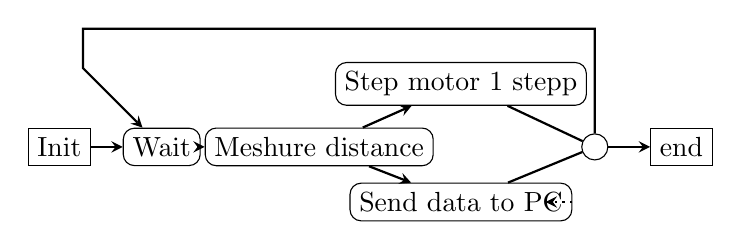
\begin{tikzpicture}
\tikzstyle{startstop} = [rectangle, rounded corners , minimum width=3mm, minimum height=1mm,text centered, draw=black]
\tikzstyle{round}=[circle, minimum width=0mm,draw=black]
\tikzstyle{first} = [rectangle, minimum width=1mm, draw=black]
\tikzstyle{empty}=[]

\usetikzlibrary{shapes.geometric, arrows}
\tikzstyle{arrow} = [thick,->,>=stealth]
\tikzstyle{dottarrow} = [thick, dotted,->,>=stealth]
\tikzstyle{noarrow}=[thick,-=,=stealth]

%nodes
\node (init) [first] {Init};
\node (wait) [startstop, right of =init, xshift=3mm] {Wait};
\node (mesh) [startstop, right of=wait, xshift=10mm] {Meshure distance};
\node (step) [startstop, right of=mesh, xshift=8mm ,yshift=8mm] {Step motor 1 stepp};
\node (send) [startstop, below of=step, yshift=-5mm]{Send data to PC};
\node (merge) [round, right of=mesh, yshift=0mm, xshift=25mm]{};
\node (end) [first, right of=merge, xshift=1mm] {end};
\node (topc) [empty, right of=send, xshift=2mm]{};

%arrows
\draw [arrow] (wait) -- (mesh);
\draw [arrow] (init) -- (wait);
\draw [arrow] (mesh) -- (step);
\draw [arrow] (mesh) -- (send);
\draw [noarrow] (send) -- (merge);
\draw [noarrow] (step) -- (merge);
\draw [dottarrow] (send) -- (topc);
\draw [arrow] (merge)  -- +(0,1.5)  -- (0.3,1.5) -- (0.3,1) -- (wait);
\draw [arrow] (merge) -- (end);
\end{tikzpicture}